\section{Results}\label{s:results}

\subsection{Analysing Features}\label{ss:sae_feat_analysis}

\begin{figure*}[t]
    \centering
    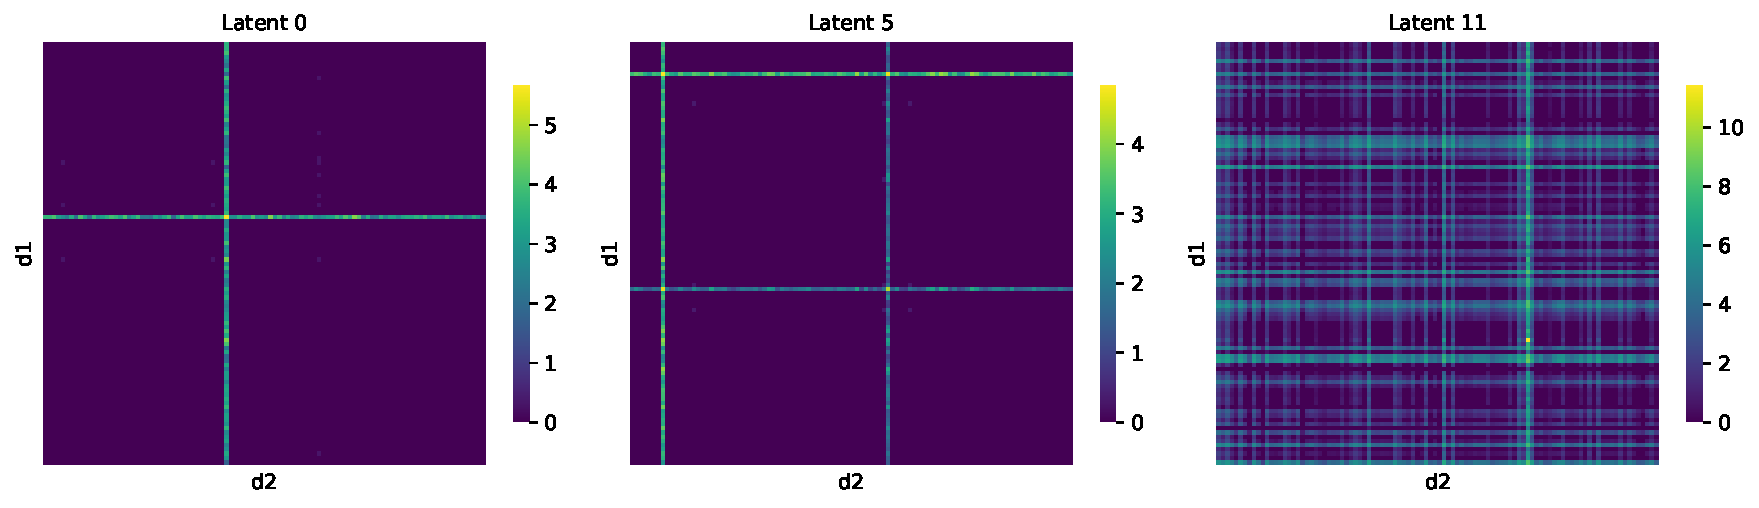
\includegraphics[width=\linewidth]{figures/sae_heatmap.pdf}
    \caption{
        These $100\times100$ heatmaps show how specific SAE latents activate for different input bigrams $(d_1, d_2)$, of which there are $100\times100$ combinations. The top-left corner cell is input $(0,0)$ and the bottom-right corner cell is $(99,99)$.
        \textbf{Left} ($1$-symbol detector): latent 0 activates only if $d_1$ or $d_2 = 41$, and activates most strongly when $d_1=d_2=41$. This results in a `plus-sign' pattern.
        \textbf{Center} ($k$-symbol detector, $k>1$): latent 5 activates only if $d_1$ or $d_2$ is either $7$ or $58$, resulting in two `plus-sign' patterns.
        \textbf{Right} (special latent): latent 11 activates for most inputs and activates much more strongly at peak than all other latents.
        }
    \label{fig:sae-heatmap}
\end{figure*} 

We plot which the activating examples for each latent on a heatmap over all inputs (Figure \ref{fig:sae-heatmap}).
We identify two latent types, excluding 8\% of latents which activate on fewer than 0.1\% of inputs: $k$-symbol detectors and special latents.

\textbf{$k$-symbol detectors (91\% of latents):} 88\% of latents are $1$-symbol detectors: they activate only if one specific symbol is present in the input at either $d_1$ or $d_2$, shown by the `plus-sign' pattern in Figure \ref{fig:sae-heatmap}. They activate most strongly where $d_1=d_2$ (the intersection), and otherwise their activation magnitude varies only with symbol presence, not position.
3\% of latents detect multiple symbols ($k>1$) and sometimes activate with different magnitudes for different symbols (e.g., latent 5 activates stronger for symbol 7 than symbol 58), suggesting magnitude carries information.

\textbf{Special latents (2 latents, 9\% of activations):} Only two latents (11 and 56) do not follow the above pattern. Latent 11 activates on 64\% of inputs and latent 56 on 9.9\%, compared to fewer than 4.5\% for all other latents (Appendix \ref{app:further_analysis}). Because they activate across most inputs, their activation cannot indicate whether a specific symbol is present, hence they are put into a `special' category.

Moreover, \citet{farrell2025order} find that $\boldsymbol r_{s}^{L_1}$ is a linear combination of input embeddings with attention weights as coefficients, so we compare correlations between activation magnitude and
\( 
\Delta \alpha = \alpha_{s \to d_1} - 
\alpha_{s \to d_2}
\), as shown in Appendix \ref{app:further_analysis}, Figure \ref{fig:alpha_diff_correlation_plot}.
Latent 11 positively correlates with $\Delta \alpha$ (Pearson correlation coefficient $r=0.807$), and latent 56 negatively correlates with $\Delta \alpha$ ($r=-0.3213$). We compute correlations over the whole dataset, and all other latents have correlation $|r| < 0.004$ with $\Delta \alpha$, suggesting that these two features are indeed special relative to the others.
% Since latent 11 strongly positively correlates with $\Delta \alpha$ we refer to it as strongly $d_1$-favouring, and we similarly refer to latent 56 as weakly $d_2$-favouring. 
Latent 11 has a much stronger correlation than 56, so we refer to it as the primary special feature.

\subsection{Steering Experiments}\label{ss:steering_exp}

We hypothesise that special latents have graded activations. Specifically, we hypothesise that they have activation ranges corresponding to different bigram orderings. To test this hypothesis, we use steering vectors \cite{ferrando2024primer,arditi2024refusal} to perform a causal linear intervention: we scale special latent activations and observe whether the model's outputs change predictably.

We: \textbf{1.} Run the transformer on bigram $(d_1, d_2)$ and record the special latent's activation magnitude $m$ from the SAE trained on $\boldsymbol r_{s}^{L_1}$.
\textbf{2.} Scale $m$ by factor $p$, reconstruct $\hat{\boldsymbol r}_{s}^{L_1}$, and compute logits at $(o_1, o_2)$.
\textbf{3.} Repeat across all $p \in [0,20]$ (step $0.05$) and all input bigrams.
Systematic output logit shifts across this sweep would imply that the special latent is graded.

% The binary view \cite{quirke2025binary} expects SAE latents to activate when a feature is present and remain inactive otherwise, with magnitude being irrelevant to the feature represented. If this were true for special latents, scaling their activation (step 2 above) would either keep outputs unchanged (same latents remain active) or produce nonsense. However, based on the circuits analysis in \citet{farrell2025order} showing that output order depends on $\Delta \alpha$, and the observation that special latents correlate with $\Delta \alpha$ (Section \ref{ss:sae_feat_analysis}), we predict that scaling these latents will cause systematic output swaps: for input $(a,b)$ where the model correctly outputs $(a,b)$, scaling the special latent may produce output $(b,a)$ at appropriate scaling factors.


Steering latent 11 produces output swaps for 5,002/10,000 bigrams (50.0\%) and an example is shown in Figure \ref{fig:steering_feat_success}. The remaining 50\% are not swapped: 3,600 inputs (36\%) where latent 11 does not activate ($m=0$), and 1,424 inputs (14.2\%) where it activates but no scaling produces a swap. The latter fail for the following reasons (see Appendix \ref{app:further_steering} for visualisations):

\textbf{Negative scaling required (9.2\%):} Swapping $o_1$ requires negative $p$, which we reject as BatchTopK activations are non-negative by construction, so negative scaling introduces an out-of-distribution anti-feature rather than representing learned graded behaviour.

\textbf{Mutually exclusive swap ranges (2.3\%):} Each output position can be individually swapped but not simultaneously.

\textbf{No swap in observed range (1.8\%):} One logit remains dominant across all $p \in [0, 20]$.

\textbf{Matching bigram elements (0.8\%):} $d_1 = d_2$, making the swap degenerate.
% NOTE
% 1) negative o1
% 2) no o2 in bounds
% 3) never predicts 2x & no o2 xover (looks same to never prdeict d1 at o2)
% 4) d1=d2

For inputs that are not swapped, it is sometimes possible to scale a co-activating (non-special) latent to successfully swap outputs (see example in Appendix \ref{app:further_steering}). 
We additionally steer latent 56 and successfully swap 2.0\% of outputs, which is part of the 36\% of inputs that do not activate latent 11 since the two special latents never coactivate. 
Although we don't steer on all latents due to computational constraints, in Appendix \ref{app:further_steering} we attempt it on several `non-special' latents to confirm the swapping behaviour is unique to latents 11 and 56.

\subsection{Generalisation to other SAEs}\label{ss:sae_generalisation}

\begin{figure*}[t]
    \centering
    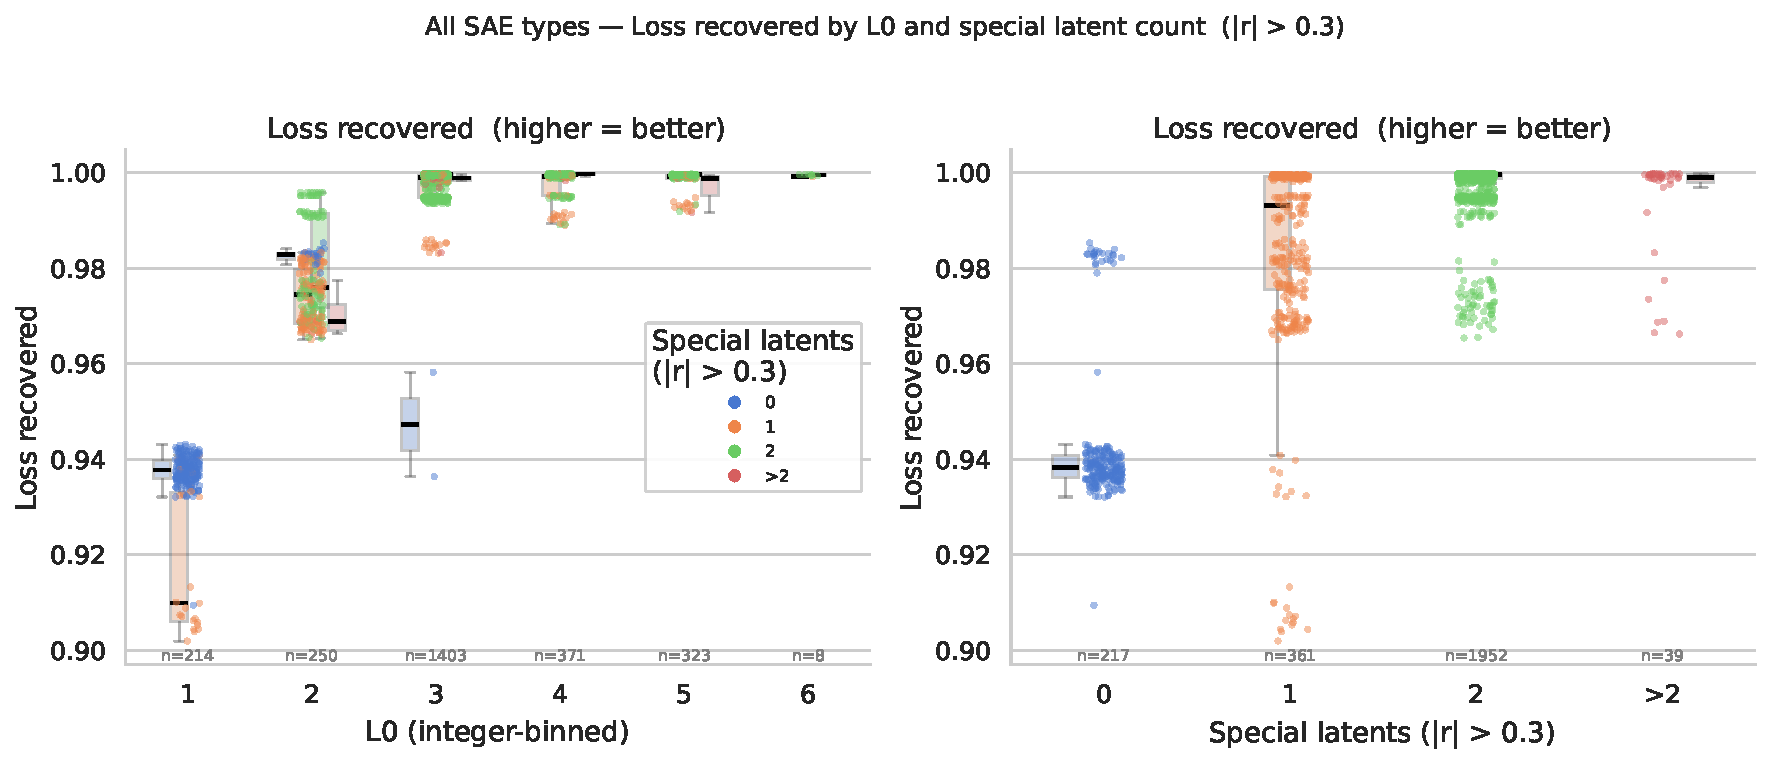
\includegraphics[width=\linewidth]{figures/special_latents_vs_performance.pdf}
    \caption{These strip plots show how the number of special latents (identified by the latent's activation's correlation with $\Delta \alpha$ using threshold $|r| > 0.3$, % TODO note that these plots actually use 0.5 so i'm lying here (can fix for actual paper but okay for now)
    as in Section \ref{ss:sae_feat_analysis}) differs across SAEs with different performance.
    It shows that SAEs with strong performance, measured by explained variance and patched cross-entropy loss, tend to have 2 special latents (spearman $r=-0.460$ for patched cross-entropy loss and $r=0.506$ for explained variance).}
    \label{fig:special_latents_vs_performance}
\end{figure*}

We test for similar behaviours in other SAEs to support generalisation of our results, albeit limited at this experimental scale.
We automatically identify special latents by checking each latent's correlation with $\Delta \alpha$ is over threshold $|r| > 0.3$. This threshold was chosen empirically because it reliably selected latents that could be steered to swap  \dots
% TODO need to run steering on ALL latents in studied model, and show table of %success AND % of successes that contained a co-acitvating 'special latent' for given thresh.


Figure \ref{fig:special_latents_vs_performance} shows that SAEs with strong performance reliably learn special latents.
This strongly suggests that the behaviour described so far in this section generalises to various SAE configurations. However, this generalisation is limited because we only tested three SAE types (BatchTopK, Matryoshka, JumpReLU) over 15 seeds. Future work should check for generalisation to more SAE variants such as those in Table \ref{tab:sae_types}, and over more training seeds for more robust statistical significance testing.
% TODO add table of different SAE sweep configs (could add to method)

% TODO could add table showing % of saes with 2 special have 1 d1 favouring the other d2 favouring (+ average corrs?). and saes with 1 special % d1 favouring and % d2 favouring + avg corrs

% NOTE currently the stats on wandb use r=0.5! not 0.3, should be consistent really

% Moreover, we test if $k$-symbol detectors appear in other SAEs
% NOTe do i need this?

% Specifically, we check the distribution of latent firing rates and identify symbol detector and special latents. We identify the latter .




% ------- steering ---

To test whether special latents can be steered to swap outputs in other SAEs, we provide the following pipeline that works given any SAE, which is available in our code repo:
\begin{enumerate}
    \item Store the SAE activations for all input bigrams by running a single 
    forward pass as in Figure \ref{fig:rq2_pipeline} over the full dataset and recording each SAE latent's activation 
    magnitude.
    \item Identify special latents using $\Delta \alpha$ correlation $|r|>0.3$ as a heuristic, 
    as described previously.
    \item For each identified special latent, run a batched steering grid search 
    over all input bigrams. For each bigram and each scale factor 
    $p \in [0,10]$ with step size 0.05 (201 values), record the logits at 
    output positions $o_1$ and $o_2$ under the steered reconstruction 
    $\hat{\boldsymbol{r}}_{s}^{L_1}$. Bigrams for which the latent does not 
    activate ($m = 0$) are skipped immediately since scaling has no effect.
    
    \item Find crossover scales for each bigram:
    \begin{itemize}
        \item For $o_1$: since $o_1$ logits are empirically linear in $p$, fit 
        lines to $\ell_{d_1}(p)$ and $\ell_{d_2}(p)$ and compute the analytical 
        intersection. Inputs for which either logit series fails an $R^2 \geq 0.999$ 
        linearity check, or for which the intersection falls on a negative scale, are flagged and excluded.
        \item For $o_2$: detect sign changes in $\ell_{d_1}(p) - \ell_{d_2}(p)$ 
        on the coarse $[0, 10]$ grid, then refine each crossing to three decimal places using 
        bisection search. All bisection tasks across the batch are executed in parallel to 
        avoid sequential per-input forward passes.
    \end{itemize}
    
    \item Determine a valid swap zone $[p_{\mathrm{lo}}, p_{\mathrm{hi}}]$ per 
    bigram by intersecting the $o_1$ and $o_2$ crossover constraints with the 
    scale ranges over which $\mathrm{argmax}(o_1) = d_2$ and 
    $\mathrm{argmax}(o_2) = d_1$ hold simultaneously. If no contiguous window 
    satisfying both conditions exists, the bigram is recorded as a failure with a 
    specific reason (see Section \ref{ss:steering_exp}).
    
    \item Verify each swap zone by running the model at the midpoint 
    $p^* = (p_{\mathrm{lo}} + p_{\mathrm{hi}})/2$ and confirming that the model 
    output is $(d_2, d_1)$.
    
    \item Report the fraction of bigrams for which a valid swap zone was found and 
    the swap verified, along with a breakdown of failure reasons for the remainder.
\end{enumerate}



Steps 3-5 of the pipeline are very computationally expensive, so we test generalisation using a varied sample of six high performing SAEs (Table \ref{tab:cherry-picked-saes}) rather than running the pipeline on all trained SAEs (as in Figure \ref{fig:special_latents_vs_performance}).
The results are shown in Table \ref{tab:steering_generalisation}.
We find that all six sampled SAEs learned at least one special latent ($|r| > 0.3$), and five learned a pair of opposing special latents (one $d_1$-favouring and one $d_2$-favouring). In every tested SAE, steering at least one of these special latents successfully swapped the predicted outputs for a substantial portion of the input space, ranging from $26.6\%$ to $72.5\%$ of all inputs. When the output swap failed, the inputs typically either did not activate the latent at all or encountered constraints similar to those detailed in Section \ref{ss:steering_exp}, such as requiring negative activation scaling. This suggests that the relative magnitude-based mechanism, and the emergence of steerable, graded latent activations, generalizes consistently across varying SAE architectures and hyperparameter configurations. In future work, this study should be extended to further configurations for robust statistical significance.